\documentclass{sig-alternate-05-2015}
\usepackage{hyperref}


\begin{document}

% Copyright
%\setcopyright{acmcopyright}
% DOI
\doi{insert doi here}

% ISBN
\isbn{insert isbn here}

\title{BigBInf Micro Cloud Platform}

\numberofauthors{1}
\author{
% 1st. author
\alignauthor
Brendan D. Ball\\
       \affaddr{University of Cape Town}\\
}

\date{30 August 2015}


\maketitle
\begin{abstract}
[Abstract]
\end{abstract}
\keywords{Big Data; BioInformatics; Clouds}


\section{Introduction}
Cloud infrastructure has the potential to simplify the processing of big data sets, as well as collaboration between remote researchers. Data could be kept in a cloud solution and researchers would execute code on the raw data.
\\
\\
Configuration of the execution environment can be time consuming, particularly in the context of bioinformatics. Cloud BioLinux is part of a cloud solution which solves this issue. This toolkit makes it easy to deploy virtual machines to a cloud platform with bioinformatics infrastructure pre-configured. It bundles specific packages used in next generation sequence analysis, thereby decreasing configuration time and increasing maintainability. Instances of Cloud BioLinux have been tested on the Amazon EC2 cloud platform and on a private Eucalyptus cloud \cite{krampis2012cloud}. 
\\
\\
Commercial clouds such as Amazon EC2, however, do not solve the problem of uploading big data sets to their cloud infrastructure \cite{baker2010next}. Micro clouds deployed on-site would overcome this challenge by keeping the data locally, while still reaping the benefits of a cloud platform. However, with different research institutions deploying their own micro clouds, cloud interoperability is required to allow researchers from different institutions to collaborate on the same data. The cloud interoperability creates a community cloud. A use-case of a specific community cloud  by Jimenez et al. \cite{jimenez2014deploying} contains core architectural properties needed for a successful community cloud. These properties include autonomy (where each micro cloud will be managed independently), security, self management of nodes, and scalability.
\\
\\
The traditional approach to creating a cloud platform allows users to run their own instances of operating systems (such as Amazon EC2) via virtualisation technology. This includes both hardware level emulation support and the software needed to manage the virtualisation. These virtualisation schemes use machine level virtualisation \cite{fink2014docker}. \\\\
A new method, known as containerization, provides much of the same functionality, with added benefits of lower resource usage and better performance. Containers are able to run native machine instructions compared to virtualisation emulating every machine instruction \cite{dua2014virtualization}. Containers are only useful when complete virtualisation is not needed, but allow for isolated application deployment and portability.
\\\\
In this work, we aim to take advantage of containers and enable efficient processing of Big Data through the use of micro clouds. We also aim to increase collaboration by connecting the micro clouds to form a community cloud.
\\\\
UCT and UWC are collaborators on this project, as is UCT E-Research. Both UWC and UCT E-Research provided valuable hardware resources enabling thorough evaluation in a real world setting.


\section{Background}

\subsection{Docker}
Docker is an implementation of a Linux container management tool. Docker functions similarly to virtualisation. It uses an image to quickly launch a pre-configured isolated environment. The key difference is that containers directly uses the Linux kernel on the host machine to run native instructions. Containers are lightweight and launched in a fraction of time of a virtual machine \cite{joy2015performance}. 
\\\\
Docker builds on Linux containers by implementing an image format which makes use of an AUFS filesystem. This allows a docker image to be built up from a number of intermediate layers. Layers can be added or removed without affecting another layer in the image \cite{boettiger2014introduction}.
\\\\
The layered approach to creating a Docker image allows images to be built using a script called a Dockerfile. Defining an image with a script makes docker images much more portable and reproducible compared to creating an image from a running environment, as is the with virtualisation \cite{boettiger2014introduction}.

\subsection{OpenStack}
To create a cloud platform which makes use of containers, we need a framework to manage containers in a cluster which will perform scheduling and resource allocation. OpenStack was the first system looked at as a base for a container manager. After much trouble trying to get it set up properly in a development environment it was decided that there are more suitable systems to solve the problem. OpenStack is very cluttered with many inter dependent components \cite{affetti2015adock}. The functionality that we require from a cluster manager for this project is limited compared to everything that OpenStack provides. Thus we looked for a smaller, simpler cluster manager to suit our needs.


\subsection{Kubernetes}
Kubernetes is purely a container manager specifically designed to orchestrate docker containers. It is still a new system and Kubernetes version 1 has just recently been released which means it is ready for production use. Using containers instead of virtual machines has only recently become popular. The growth in popularity has resulted in a number of systems being developed which provide some overlapping functionality to Kubernetes. Kubernetes looks most promising as it is easy to use. Given that it is relatively new it is not cluttered and aims to solve a single problem of being a container manager \cite{googleborg}. 


\section{Design}


\subsection{Design Aims}
The aim is to form a community cloud which will allow sharing of data and collaboration of users between multiple micro clouds.
\\\\
Users will access data and submit jobs by interacting with a front end web interface. The functionality of the platform is of primary concern, thus user interface design will not be considered and is outside the scope of this project. 
\\\\
As multiple jobs can be submitted by multiple people, these jobs have to be scheduled properly to allow successful completion of each job. 


\subsection{Constraints}
Micro cloud deployments for evaluation are limited to UWC and UCT E-Research. The evaluation is limited to one community cloud containing two micro clouds.

\subsection{Software Engineering}

We implemented a proof of concept of the community cloud. The aim was not to focus on software engineering methodologies. However to allow for reproducibility the source code is stored in a Git repository hosted on Github (Git is a version control system). 

\subsubsection{Micro Cloud Components}
The platform consists of the follwing components: a web interface, a scheduler, an image builder and image repository, a cluster manager (the master node), multiple worker nodes, and a storage interface which allows reading from and writing to persistent storage. Figure \ref{fig:architecture} shows the connection between components.

\begin{figure}
\centering
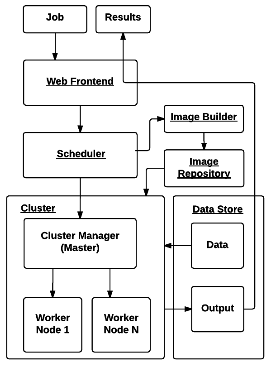
\includegraphics[scale=0.8]{img/microcloud_architecture}
\caption{Micro Cloud Architecture}
\label{fig:architecture}
\end{figure}

\subsection{Evaluation}
The functionality of the micro cloud is evaluated by submitting sample analysis code as a job. The analysis code searches against a genome database from NCBI's NR database which is publicly available \cite{pruitt2005ncbi}. The analysis code makes use of the BLAST+ search tool \cite{camacho2009blast}. The code itself consists of custom queries. Different sized jobs are tested by increasing or decreasing the size of the query, which makes it easily scalable to different sized test cases.



\subsection{Implementation}


A job describes a single instance of code uploaded for execution. 
The micro cloud platform uses containers, more specifically Docker containers to execute code. Docker images are created with dockerfiles which specify the execution environment and what files to execute. Submitting a job requires a Dockerfile and source code to be executed, uploaded together packaged as a single tarball.  

\subsubsection{Cluster Manager - Kubernetes}
In this project cluster manager is synonomous with container manager because the cluster will strictly operate by running containers. Kubernetes has been chosen as the cluster manager framework for managing the micro cloud.

\subsubsection{Docker Images}
A dedicated docker-in-docker container is run which is used to build docker images from dockerfiles. The image is then pushed to a private docker repository which can be accessed by any node in the cluster. The docker image is pulled by a worker node when the job is assigned to that worker node.

\subsubsection{Scheduler}
The default scheduler will rely on a first-in-first-out (FIFO) queue to schedule jobs. There are two parts to the scheduler. The first part schedules new jobs' images to be built from the Dockerfiles. The second part schedules the jobs to be executed on one of the worker nodes.

\subsubsection{Storage}
The cluster at UWC which the micro cloud will be tested on makes use of Ceph storage which can be accessed by a RADOS Block Device (RBD). Kubernetes already provides support for mounting an RBD as a storage volume in a container.

\subsubsection{Web Interface}
The backend web interface will be implemented using the python flask web framework. It is a minimalist framework which allows for rapid development of web interfaces. 
The front end web interface will be implemented using Angularjs to create a single page application. 
draw
\subsubsection{Community Cloud}
A community cloud will be formed by implementing a centralised discovery service. This will improve scalability compared to a full mesh network between micro clouds.



\bibliographystyle{ACM-Reference-Format-Journals}
\bibliography{ref} 


\end{document}
